\documentclass[review]{elsarticle}

\usepackage{lineno,hyperref}
\usepackage{graphicx}
\usepackage[labelfont=bf]{caption}
\usepackage[utf8]{inputenc}
\usepackage[T1]{fontenc}
\usepackage{subcaption}
%\usepackage[latin1]{inputenc}
\usepackage{pifont} 
\usepackage{import}
\usepackage{amsmath}
\usepackage{multirow}
\usepackage{graphicx,url}
\usepackage{placeins}
\usepackage{adjustbox}
\usepackage[english]{babel}
\usepackage{lipsum}
\usepackage{multicol}
\usepackage{textcomp}
\usepackage{listings}
\usepackage[svgnames]{xcolor}
\usepackage[framemethod=TikZ]{mdframed}
\usepackage{caption}
\usepackage{amsmath}
\usepackage{calc}
\usepackage{array,url,kantlipsum}
\usepackage{algorithm}
\usepackage{algpseudocode}
\usepackage{lscape}
\usepackage{array}
\usepackage{longtable}
\usepackage[inline]{enumitem}
\usepackage{booktabs}
\usepackage{txfonts}
\usepackage{soul}
\usepackage{colortbl}%
  \newcommand{\myrowcolour}{\rowcolor[gray]{0.925}}
\newenvironment{Figure}
  {\par\medskip\noindent\minipage{\linewidth}}
  {\endminipage\par\medskip}

\lstset{
language=Java,
basicstyle=\small\ttfamily,
numbers=left,
numbersep=5pt,
xleftmargin=20pt,
frame=tb,
framexleftmargin=20pt
}


\modulolinenumbers[5]

\journal{Journal of \LaTeX\ Templates}

%%%%%%%%%%%%%%%%%%%%%%%
%% Elsevier bibliography styles
%%%%%%%%%%%%%%%%%%%%%%%
%% To change the style, put a % in front of the second line of the current style and
%% remove the % from the second line of the style you would like to use.
%%%%%%%%%%%%%%%%%%%%%%%

%% Numbered
%\bibliographystyle{model1-num-names}

%% Numbered without titles
%\bibliographystyle{model1a-num-names}

%% Harvard
%\bibliographystyle{model2-names.bst}\biboptions{authoryear}

%% Vancouver numbered
%\usepackage{numcompress}\bibliographystyle{model3-num-names}

%% Vancouver name/year
%\usepackage{numcompress}\bibliographystyle{model4-names}\biboptions{authoryear}

%% APA style
%\bibliographystyle{model5-names}\biboptions{authoryear}

%% AMA style
%\usepackage{numcompress}\bibliographystyle{model6-num-names}

%% `Elsevier LaTeX' style
\bibliographystyle{elsarticle-num}
%%%%%%%%%%%%%%%%%%%%%%%

\begin{document}

\begin{frontmatter}

\title{Search-Based Stress Testing with Multiobjective Evolutionary Algorithms: A Comparative Case Study }

%% Group authors per affiliation:
\author[mymainaddress]{Nauber Gois}
\fntext[myfootnote]{Since 1880.}

%% or include affiliations in footnotes:
\author[mymainaddress]{Pedro Porfírio}
\ead[url]{www.elsevier.com}

\author[mymainaddress]{André Coelho}
\cortext[mycorrespondingauthor]{Corresponding author}
\ead{support@elsevier.com}

\address[mymainaddress]{Universidadede Fortaleza. Av. Washington Soares, 1321 - Edson Queiroz, Fortaleza - CE, 60811-905}


\begin{abstract}
Some software systems must respond to thousands or millions of concurrent requests. Performance degradation and consequent system failures usually arise in stressed conditions. Stress testing subjects the program to heavy loads. Stress tests differ from other kinds of testing in that the system is executed on its breakpoints, forcing the application or the supporting infrastructure to fail. The search for the longest execution time is seen as a discontinuous, nonlinear, optimization problem, with the input domain of the system under test as a search space. In this context, search-based testing is viewed as a promising approach to verify timing constraints. Search-based software testing is the application of metaheuristic search techniques to generate software tests. The test adequacy criterion is transformed into a fitness function and a set of solutions in the search space is evaluated with respect to the fitness function using a metaheuristic. Multi-objective heuristics may be more suitable for non-functional search-based tests since these tests usually aim to obtain a result with more than one objective. This paper investigates the use of the multi-objective NSGA-II, SPEA2, PAES and MOEA/D algorithms in search-based stress testing. MOEA/D metaheuristics obtained the best hypervolume value when compared with other approaches. 

\end{abstract}

\begin{keyword}
Search-based Stress Testing\sep Multi-objective algorithms \sep Elsevier \sep template
\MSC[2010] 00-01\sep  99-00
\end{keyword}

\end{frontmatter}

\linenumbers

\section{Introduction}

Performance problems such as high response times in software applications have a significant effect on the customers’  satisfaction. The explosive growth of the Internet has been instrumental in the increased need of applications that perform at an appropriate speed. Moreover, performance problems are often detected late in the application life cycle, and the later they are discovered, the greater the cost is to fix them. The use of stress testing is an increasingly common practice owing to the increasing number of users. In this scenario, the inadequate treatment of a workload,  generated by concurrent or simultaneous access due to several users, can result in highly critical failures and negatively affect the customers' perception of the company  \cite{Jiang2010} \cite{Molyneaux2009} \cite{Wert2014}.

Software testing is an expensive and difficult activity. The exponential
growth in the complexity of software makes the cost of testing continue to grow. Test case generation can be viewed as a search problem. The test adequacy criterion is transformed into a fitness function and a set of solutions in the search
space are evaluated with respect to the fitness function using a metaheuristic search technique. Search-based software testing is the application of metaheuristic search techniques to generate software
tests cases or perform test executions \cite{Afzal2009a}.

Software performance is a pervasive quality,  because it is influenced by every aspect of the design, code, and execution environment. Performance failures occur when a software product is not able to meet its overall objectives due to inadequate performance. Such failures negatively impact the projects by increasing costs, decreasing revenue or both \cite{Vetoio2011}. Stress testing of enterprise applications is manual, laborious, costly, and not particularly effective. When running many different test cases and observing application’s behavior, testers intuitively sense that there are certain properties of test cases that are likely to reveal performance bugs \cite{Grechanik2012}. Manual analysis of load testing is inefficient and error prone due to incomplete knowledge of test analyst about the application under test\cite{Arslan2015}.

Stress testing is an expensive and difficult activity. The exponential
growth in the complexity of software makes the cost of testing has only continued continued to grow. Test case generation can be seen as a search problem. The test adequacy criterion is transformed into a fitness function and a set of solutions in the search
space are evaluated with respect to the fitness function using a metaheuristic search technique. Search-based software testing is the application of metaheuristic search techniques to generate software
tests cases or perform test execution \cite{Afzal2009a}.

Search-based stress testing (SBST) is regarded as a promising approach to verify timing constraints \cite{Afzal2009a}. A common objective of a load search-based test is to find  scenarios that produce execution times that violate the specified timing constraints \cite{Sullivan}. 

Usually, search-based test methods are based on a single objective optimization. Multi-objective evolutionary algorithms (MOEAs) are commonly used for solving multi-objective problems (MOPs) because they produce a complete set of solutions in a single run. Consequently, multi-objective heuristics may be more suitable in non-functional search-based tests, since these tests usually aim to obtain a result with more than one objective, for example, maximize the number of users of an application, minimizing your response time. 


The present study extends the article "Improving stress search based testing using a hybrid metaheuristic approach"  \citep{Gois2016} in order to ascertain if the use of multi-objective algorithms in search-based stress testing. This paper  addresses the following  research question:

\begin{itemize}
\item Which, among the four algorithms chosen, is the most suitable multi objective algorithm for the search-based test problem?
\end{itemize}

One experiment was conducted to validate the proposed approach. The  experiment was performed using an installed JPetStore application. The experiment presents the experimental results to compare four multi-objective algorithms in search-based stress testing. 

The remainder of the paper is organized as follows. The next section gives background on multi-objective metaheuristics. Section 3 presents presents the Hybrid approach proposed by Gois et al. \citep{Gois2016}. Section 4 presents the comparative experiment performed.  Conclusions and further work are presented in Section 5.

\section{Multi-objective optimization using evolutionary algorithms}

Many real optimization problems require optimizing multiple conflicting objectives. There is no single optimal solution, but a set of alternative solutions. The objectives that have to be optimized are often in competition with one another and may be contradictory; we may find ourselves trying to balance the different optimization objectives of several distinct goals \cite{Harman2010}. The image of all the efficient solutions is called the Pareto front or Pareto curve or surface. The shape of the Pareto surface indicates the nature of the trade-off between the different objective functions. An example of a Pareto curve is reported in Fig. \ref{fig:pareto1}. Multi-objective optimization methods have as main purposes to minimize the distance between the nondominated front and the Pareto optimal front and find a set of solutions that are as diverse as possible.

\begin{figure}[h]
\centering
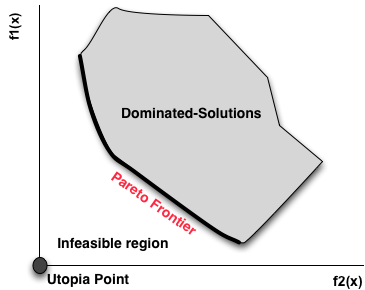
\includegraphics[width=0.4\textwidth]{./images/paretofront.png}
\caption{An optimized Pareto front example}
\label{fig:pareto1}
\end{figure}

What distinguishes multi-objective evolutionary algorithms from single objective metaheuristics is how they rank and select individuals in the population. If there is only one objective, individuals are naturally ranked according to this objective, and it is clear which individuals are best and should be selected as
parents. In the case of multiple objectives, it is still necessary to rank the individuals, but it is no longer obvious how doing this. Most people probably agree that a good approximation to the Pareto front is characterized by:

\begin{itemize}
\item  a small distance of the solutions to the true Pareto frontier,
\item  a wide range of solutions, i.e., an approximation
of the extreme values, and
\item a good distribution of solutions, i.e., an even
spread along the Pareto frontier.
\end{itemize}

The approximation of the Pareto-optimal set involves itself two objectives: minimize the distance to the optimal front and maximize the diversity of the generated solutions. There are two fundamental issues when designing a multiobjective evolutionary algorithm: mating selection and environmental selection. The first issue is related to the question of how to guide the search towards the Pareto-optimal front. The procedure to fill the mating pool is usually randomized. The second issue is related to the question of which individuals to keep during the evolution process. In most modern multi-objective algorithms these two concepts are realized in the following way: Environmental selection or Mating selection \cite{Zitzler2001}.

In  Environmental selection, an archive is maintained which contains a representation of the nondominated front among all solutions considered so far. A member of the archive is only removed if i) a solution has been found that dominates it or ii) the maximum archive size is exceeded and the portion of the front where the archive member is located is overcrowded \cite{Zitzler2001}.

In Mating selection, the pool of individuals is evaluated in two phases. First, all individuals are compared on the basis of the Pareto dominance. Basically, the information which individuals each individual dominates, is dominated by or is indifferent to is used to define a ranking on the generation pool. Afterwards, this ranking is refined by the incorporation of density information. Various density estimation techniques are used to measure the size of the niche in which a specific individual is located \cite{Zitzler2001}.


\subsection{NSGA-II: Nondominated Sorting Genetic Algorithm II}

Multi-objective metaheuristics rank individuals according to the defined goals. Deb et al. proposed the Nondominated Sorting Genetic Algorithm II (NSGA-II) algorithm taking into account the need to reduce computational complexity in non-dominated classification while introducing elitism and eliminating subjectivity in the allocation of the sharing parameter \cite{Deb2000}. NSGA-II is a multi-objective algorithm, based on GAs, and implements the concept of dominance, in other words, to classify the total population in fronts according to the degree of dominance. According to NSGA-II, the individuals that are located on the first front are considered the best solutions of that generation, while in the last front are the worst. Using this concept, one can find more consistent results, located closer to the Pareto region, and better adapted to the type of problem.

The NSGA algorithm II applies a fitness evaluation in an initial population (Figure \ref{fig:nsga2}- \ding{202} and \ding{203}). The populations are ranked using multiple tournament selections, which consist of comparing two solutions (Figure \ref{fig:nsga2}- \ding{204}). In order to estimate the density of the solutions surrounding a particular solution in the population, the common distance between the previous solution and the posterior is calculated for each of the objectives. This distance serves as an estimate of the size of the largest cuboid that includes solution i without including any other solution of the population. A solution i beats another solution if:

\begin{itemize}
\item Solution i has a better rank, then $Rank_i$ <$Rank_j$.
\item Both solutions have the same rank, but i has a greater Distance than j, then $Rank_i$ = $Rank_j$ and $Distance_i$>$Distance_j$.
\end{itemize}

At the end of each analysis a certain group of individuals is classified as belonging to a specific category called the front, and upon completion of the classification process, all individuals will be inserted into one of the n fronts. Front 1 is made up of all nondominated solutions. Front 2 can be achieved by considering all nondominated solutions excluding solutions from front 1. For the determination of front 3, solutions previously classified on front 1 and 2 are excluded, and so on until all individuals have been classified on some front.

After selection, recombination and mutation are performed as in conventional GAs (Figure \ref{fig:nsga2}- \ding{205}). The two sets (father and son of the same dimension) are united in a single population (dimension 2) and the classification is applied in dominance fronts. In this way, elitism is guaranteed preserving the best solutions (fronts are not dominated) in the latest population (Figure \ref{fig:nsga2}- \ding{207}).

However, not all fronts can be included in the new population. Thus, Deb et al. proposed a method called crowd distance, which combines the fronts not included in the set, to compose of the last spaces of the current population, guaranteeing the diversity of the population \cite{Deb2000}. The NSGA-II algorithm creates a set of front lines, in which each front containing only non–dominating solutions. Within a front, individuals are rewarded for being ‘spread out’. The algorithm also ensures that the lowest ranked individual of a front still has a greater fitness value than the highest ranked individual of the next front \cite{Yoo2007}.




\begin{figure}[h]
\centering
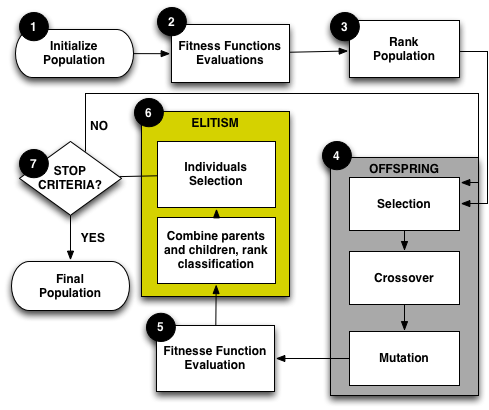
\includegraphics[width=0.5\textwidth]{./images/NSGA-2.png}
\caption{NSGA-II Algorithm}
\label{fig:nsga2}
\end{figure}

\subsection{SPEA2: Strength Pareto Evolutionary Algorithm}

SPEA uses a regular population and an archive. Starting with an initial population and an empty archive the following steps are performed per iteration. First, all non-dominated population members are copied to the archive; any dominated individuals or duplicates are removed. If the size of the updated archive exceeds a predefined limit, further archive members are deleted by a clustering technique which preserves the characteristics of the non-dominated front. Afterwards, fitness values are assigned to both archive and population members. Each individual i in the archive assign a strength value S(i) $\in$ [0, 1], which at the same time represents its fitness value F(i). 0 indicates a non-dominated individual,whereas a high value points out that the individual is dominated by many other ones. S(i) is the number of population members j that are dominated by or equal to i with respect to the objective values, divided by the population size plus one. The algorithmic framework of SPEA2 is described in Alg. \ref{spea2}. An initial population $P_{0}$ and an initial archive are created. The fitness value of all individuals is calculated in population and in the archive (external set). All non-dominated individual are copied to the new archive. Finally, the algorithm select the individual using a tournament selection \cite{Zitzler2001} \cite{Tervonen2017} \cite{MatneiFilho2016}.

\begin{algorithm}[h]
  \caption{SPEA2 Algorithm \cite{Zitzler2001}}\label{spea2}
  \begin{algorithmic}[1]

    \State Read N - Population size
    \State Read $ \overset{-}{N}$ - Archive size
    \State Read T - Maximum number of generations
    \State Generate a initial population $P_{0}$
    \State Create a initial archive $ \overset{-}{P} $
    \State Set T to zero
    \State Calculate the fitness value of individuals in $P_{t}$
    \State Calculate the fitness value of individuals in $\overset{-}{P}_{t}$
    \State Environmental Selection - Copy all non-dominated individuals in $P_{t}$ and $\overset{-}{P}_{t}$  to $\overset{-}{P}_{t+1}$
    \If {size of  $\overset{-}{P}_{t+1}$ exceeds  $ \overset{-}{N}$ }
    \State reduce  $\overset{-}{P}_{t+1}$ by means of truncation operator
    \ElsIf { size of  $\overset{-}{P}_{t+1}$ less than  $\overset{-}{N}$ }
    \State fill $\overset{-}{P}_{t+1}$ with dominated individuals in $P_{t}$ and $\overset{-}{P}_{t}$
    \EndIf
    \If {t $\gg$ T or another stopping criterion is satisfied }
    \State set A to the set of decision vectors represented by non-dominated individuals in $\overset{-}{P}_{t+1}$
    \State Stop
    \EndIf
    \State Mating selection - Perform binary tournament selection with replacement on $\overset{-}{P}_{t+1}$ in order to fill the mating pool
  \end{algorithmic}
\end{algorithm}

The main differences between SPEA2 and NSGA-II are the diversity assignment and replacement. NSGA-II uses a fast non-dominated sorting algorithm and uses Pareto optimal levels as the primary criterion to select solutions. SPEA2 derives the strength of each solution from the number of other solutions it dominates. NSGA-II uses the crowding-distance to maintain a well-spread set of solutions whereas SPEA2 applies the k-nearest neighbor approach (Figure \ref{fig:speansga}) \cite{Tervonen2017} \cite{Deb2005}.


\begin{figure}[h]
\begin{minipage}{.6\textwidth}
\centering
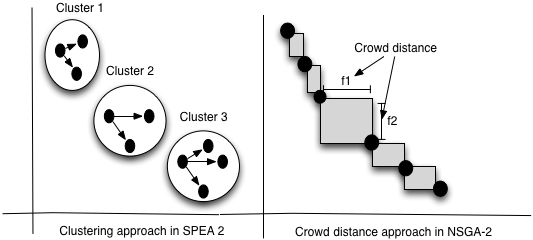
\includegraphics[width=1\textwidth]{./images/speansga.png}
\caption{Comparison between SPEA-2 and NSGA-II \cite{Deb2005}}
\label{fig:speansga}
\end{minipage}
\begin{minipage}{.4\textwidth}
\centering
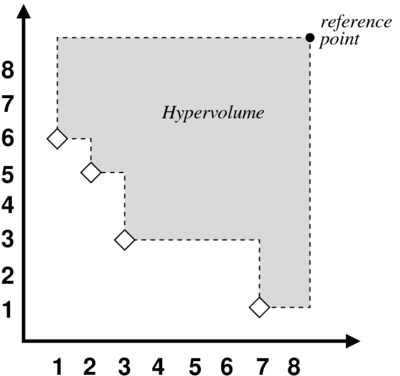
\includegraphics[width=0.7\textwidth]{./images/hypervolume-annot.png}
\caption{Hypervolume metric \cite{Lacour2015}}
\label{fig:hypervolume}
\end{minipage}
\end{figure}


\subsection{PAES: Pareto Archived Evolution Strategy} 

Pareto Archived Evolution Strategy (PAES) is an  evolutionary algorithm which employs
local search for the generation of new candidate solutions but
utilises population information in its selection procedure. The PAES algorithm was developed with two main objectives. The first of these was that the algorithm should be strictly confined to local search i.e. it should use a small change (mutation) operator only, and move from a current solution to a nearby neighbour. The second objective was that the algorithm should be a true Pareto optimiser, treating all non-dominated solutions as having equal value \cite{Knowles1999}. In PAES one parent generates by mutation one
offspring. The offspring is compared with the parent. If the offspring dominates the parent, the offspring is accepted as
the next parent and the iteration continues. If the parent dominates the offspring, the offspring is discarded and the new mutated solution (a new offspring) is generated. If the offspring and the parent do not dominate each other, a comparison set of previously non-dominated individuals is used \cite{Knowles1999}\cite{Oltean2005}. The algorithmic framework of PAES is described in Alg. \ref{paes}.


\begin{algorithm}[h]
  \caption{PAES Algorithm \cite{Knowles1999}\cite{Oltean2005}}\label{paes}
  \begin{algorithmic}[1]
    \State Repeat until a termination criterion has been reached
    \State Generate initial random solution c and add it to archive
    \State Mutate c to produce m and evaluate m
    \If {c dominates m }
    \State discard m
    \Else
    \If {m dominates c}
     \State replace c with m and add m to the archive
    \Else
    \If {m is dominated by any member of the archive}
    \State discard m
    \Else
    \State apply test (c, m, archive) to determine which becomes the new current solution and whether to add m to the archive
    \EndIf
    \EndIf
    \EndIf
  \end{algorithmic}
\end{algorithm}

\subsection{MOEA/D: A Multiobjective Evolutionary Algorithm Based on Decomposition}

The Multiobjective Evolutionary Algorithm Based on Decomposition (MOEA/D) is a multiobjective evolutionary algorithm competitive to other well-known multiobjective optimization evolutionary algorithms (MOEAs) such as NSGA-II or SPEA-2 \cite{Michalak2014}. MOEA/D decomposes a multiobjective optimization problem into a number of scalar optimization subproblems and optimizes them simultaneously. Each subproblem is optimized by only using information from its several neighboring subproblems, which makes MOEA/D have lower computational complexity at each generation than MOGLS and non-dominated sorting genetic
algorithm II (NSGA-II) \cite{Zhang2007}. 

NSGA-II, SPEA2 and PAES algorithms  do not associate each individual solution with
any particular scalar optimization problem. In a scalar objective optimization problem, all the solutions can be compared based
on their objective function values and the task of a scalar objective evolutionary algorithm (EA) is often to find one single
optimal solution. MOEA/D explicitly decomposes the problem into scalar optimization subproblems.It solves these subproblems simultaneously by evolving
a population of solutions. At each generation, the population is
composed of the best solution found so far for each subproblem. The neighborhood relations among these subproblems are defined based on the distances between their aggregation coefficient vectors \cite{Zhang2007} \cite{McConaghy2011}. Fig. \ref{fig:moead} MOEA/D create a set of subproblems $W_{i}$. Each subproblem $W_{i}$ is improved to obtain the Pareto frontier \cite{McConaghy2011}. 


\begin{figure}[h]
\centering
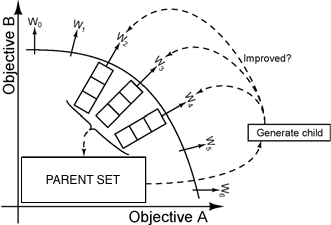
\includegraphics[width=0.5\textwidth]{./images/moead.png}
\caption{MOEA/D algorithm subproblems \cite{McConaghy2011}}
\label{fig:moead}
\end{figure}

The Alg. \ref{moead} presents the details of the algorithm. The algorithm  includes the
use of Tchebycheff approach as the decomposition method, with dynamical resource allocation, to improve the efficiency of the MOEA/D \cite{Yuen2009}. 

\begin{algorithm}[!h]
  \caption{MOEA/D Algorithm}
  \label{moead}
  \begin{algorithmic}[1]
    \State \textbf{Initialization}
    \State Generate initial population by uniformly spreading and randomly sampling from search space
    \State Calculate the reference point for the Tchebycheff approach.
   \State Evaluate Objective Values 
   \State Selection using tournament selection method 
   \State Selection of mating and updating range
   \State Reproduction
   \State Repair
   \State Update of solutions 
   \State \textbf{Update}
   \State While (not equal to termination condition)
  \State Evaluate Objective Values
  \State Selection using tournament selection method
  \State Selection of mating and update range
  \State Reproduction
  \State Repair - if the searching element is out of boundary
  \State Update the solutions 
  \State \textbf{Stopping Criteria}
  \If {generation is a multiplication of a pre-set value of x}
  \State Update utility function;
  \EndIf    
  \end{algorithmic}
\end{algorithm}


\subsection{Comparing Multi-Objective Metaheuristics}

Deb states that are two orthogonal goals for any multi-objective algorithm \cite{deb2001multi}:

\begin{itemize}
\item Identify solutions as close as possible  to the true Pareto frontier;
\item identify a diverse of sets of solutions distributed across the entire Pareto-optimal surface.
\end{itemize}

There are several metrics either closeness or diversity. Example of metrics which measure the closeness of Pareto frontier is Error ratio and Set coverage. Example of metrics which measure the diversity are the Spacing and the Spread. The Hypervolume metric measure both closeness and diversity \cite{janssens2010multiple}. The Hypervolume metric calculates the volume in an objective space covered by the non-dominated individuals. The hypervolume was originally proposed by Zitzler and Thiele \cite{Zitzler1999}. It is especially useful when the true Pareto-optimal solution is unknown. For each solution, a hypercube is computed from a reference point and the solution as the diagonal corners of the hypercube ( Figure \ref{fig:hypervolume} ) \cite{janssens2010multiple}. The reference point is found by constructing a vector of worst objects fitness value.

\subsection{Noise Reduction}

Software is pervasive, which raises the value of testing it \cite{Sandler2004}. Various actions outside the application under test can cause high response times such as pagination, network usage or even a software upgrade. It is necessary a noise reduction strategy in stress test in this situations. Noisy optimization is currently receiving increasing popularity for its widespread applications in engineering optimization
problems, where the objective functions are often found to be contaminated with noisy \cite{Rakshit2017}. 


Standard Error Dynamic Resampling (SEDR), the strategy has been employed for solving both noisy single and multi-objective evolutionary
optimization problems. The working principle of SEDR is to add samples to a solution sequentially until the standard error of
the objectives fall below a chosen threshold value \cite{Siegmund2013}. It was proposed in \cite{DiPietro2004} for single-objective optimization problems. In this study, we apply SEDR on multi-objective problems by aggregating all objective values to a scalar value. As aggregation, the median of the objective standard errors is used. The strategy is concerned with the optimal allocation of sampling budget to a trial solution based on the noise strength at its corresponding position in the search space. The contamination level of noise is captured by the standard error of the mean fitness estimate of a trial solution. The SEDR algorithm is described in Alg. \ref{SEDR}.


\begin{algorithm}[h]
  \caption{SEDR algorithm \cite{Siegmund2013}}\label{SEDR}
  \begin{algorithmic}[1]

    \State \textbf{input :} Solution s
    \State Draw $b_{min}\ge 2$ initial samples of s, F(s)
    \State Calculate mean of the available fitness for each of the \textit{m} objectives: $\mu_{i}(s)$, i=1,...,m
    \State Calculate standard deviation: $\sigma_{i}=\sqrt{ \frac{1}{n-1} \sum_{n}^{j=1} (F^i_{j}-\mu_{i}(s))^2} $
    \State Calculate the standard error: $se_{i}(s)=\frac{\sigma_{i}}{\sqrt{n}}$
    \State Calculate an aggregation of the standard errors $\overline{se}(s)$
    \State Stop if  $\overline{se}(s)$ > threshold or $b_{s}\ge b_{max}$ otherwise go to step 2
  \end{algorithmic}
\end{algorithm}

\section{Improving Stress Search Based Testing using Hybrid Metaheuristic Approach}

This section presents the Hybrid approach proposed by Gois et al. \citep{Gois2016}. The solution proposed by Gois et al. makes it possible to create a model that evolves during the test. A plugin called iadapter was implemented for the research. IAdapter is a JMeter plugin designed to perform search-based stress tests.  The plugin is available at \url{www.github.com/naubergois/newiadapter}.  


The proposed solution model uses genetic algorithms, tabu search, and simulated annealing in two different approaches. The study initially investigated the use of these three algorithms. Subsequently, the study will focus on other population-based and single point search metaheuristics. The first approach uses the three algorithms independently, and the second approach uses the three algorithms collaboratively (hybrid metaheuristic approach).

In the first approach , the algorithms do not share their best individuals among themselves. Each algorithm evolves in a separate way (Fig. \ref{fig:firstaproach}). The second approach uses the algorithms in a collaborative mode (hybrid metaheuristic). In this approach, the three algorithms share their best individuals found (Fig. \ref{fig:secondapproach}). The next subsections present details about the used metaheuristic algorithms (Representation, initial population and fitness function).


\subsection{Representation}

The solution representation provides a common representation for all workloads. Each workload is composed by a linear vector with 21 positions (Figure \ref{fig:solution}  -\ding{202}). The first position represents an metadata with the name of an individual. The next positions represent 10 scenarios and their numbers of users (Figure \ref{fig:solution}  -\ding{203}). The fixed-length genome approach was chosen in reason of the ease of implementation in the JMeter tool. Each scenario is an atomic operation: the scenario must log into the application, run the task goal, and undo any changes performed, returning the application to its original state. 

Figure. \ref{fig:solution} presents the solution representation and an example using the crossover operation. In the example, solution 1 (Figure \ref{fig:solution}  -\ding{204}) has the Login scenario with 2 users, the Search scenario with 4 users, Include scenario with 1 user and the Delete scenario with 2 users.  After the crossover operation with solution 2 (Figure \ref{fig:solution}  -\ding{205}), We obtain a solution with the Login scenario with 2 users, the Search scenario with 4 users, the Update scenario with 3 users and the Include scenario with 5 users (Figure \ref{fig:solution}  -\ding{206}). Figure. \ref{fig:solution} -\ding{207} shows the strategy used by the proposed solution to  obtain the neighbors for the Tabu search and simulated annealing algorithms. The neighbors are obtained by the modification of a single position (scenario or number of users) in the vector.



\begin{figure}[h]
\begin{minipage}{.5\textwidth}
\centering
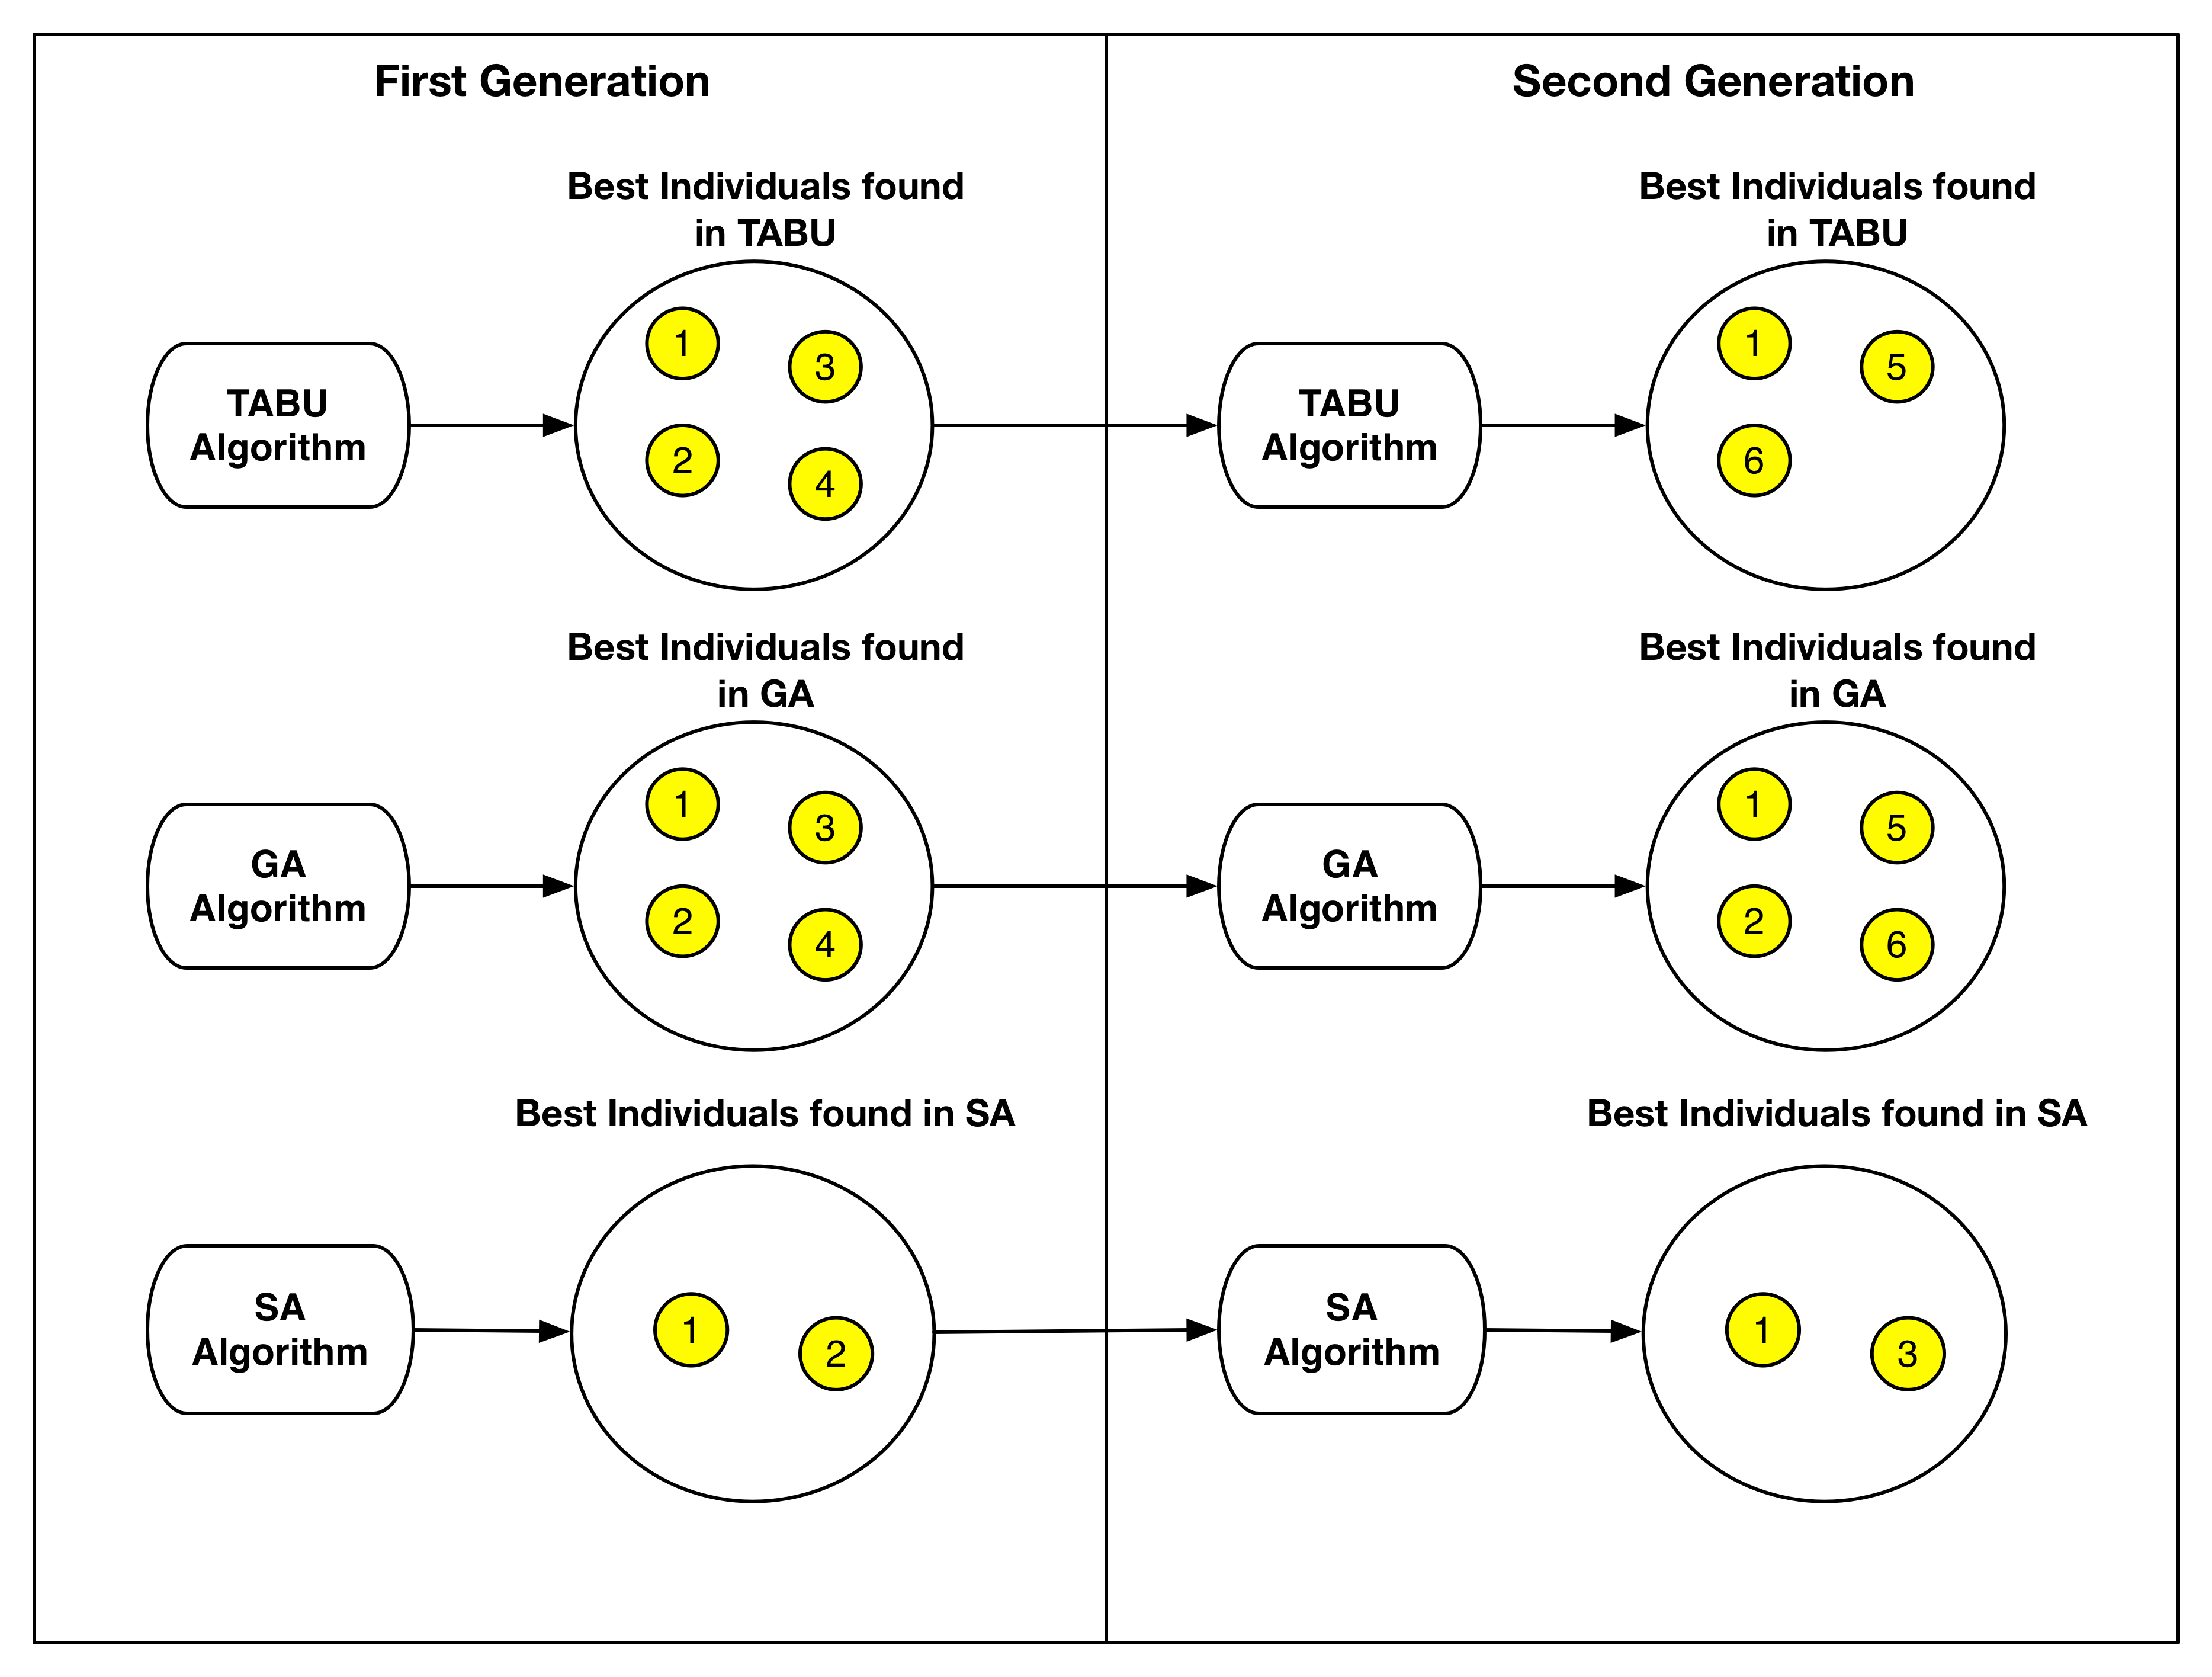
\includegraphics[width=1\textwidth]{./images/independ.png}
\caption{Use of the algorithms independently \citep{Gois2016}}
\label{fig:firstaproach}
\end{minipage}
\begin{minipage}{.5\textwidth}
\centering
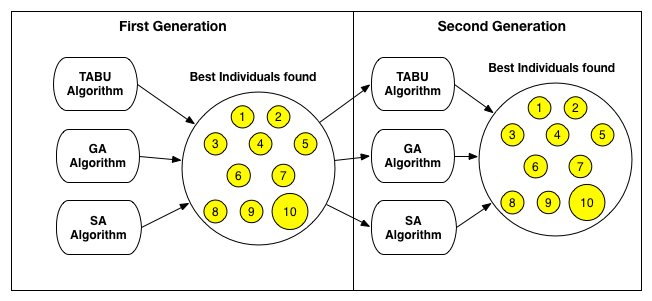
\includegraphics[width=1\textwidth]{./images/collaborative.png}
\caption{Use of the  algorithms collaboratively \citep{Gois2016}}
\label{fig:secondapproach}
\end{minipage}
\end{figure}


\begin{figure}[h]
\centering
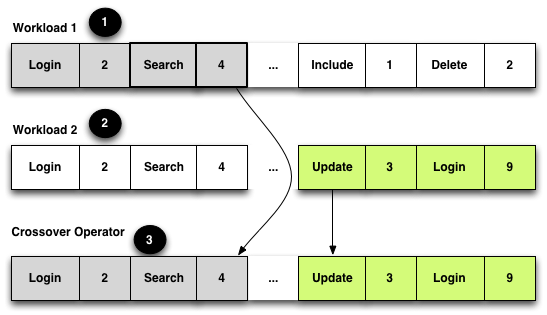
\includegraphics[width=1\textwidth]{./images/genomere.png}
\caption{Solution representation, crossover  and neighborhood operators \citep{Gois2016}}
\label{fig:solution}
\end{figure}


\subsection{Initial population}

The strategy used by the plugin to instantiate the initial population is to generate 50\% of the individuals randomly, and 50\% of the initial population is distributed in three ranges of values:

\begin{itemize}
\item Thirty percent of the maximum allowed users in the test;
\item Sixty percent of the maximum allowed users in the test; and
\item Ninety percent of the maximum allowed users in the test.
\end{itemize}

The percentages relate to the distribution of the users in the initial test scenarios of the solution. For example, in a hypothetical test with 100 users, the solution will create initial test scenarios with 30, 60 and 90 users.

\subsection{Objective (fitness) function}

The proposed solution was designed to be used with independent testing teams in various situations, in which the teams have no direct access to the environment, where the application under test was installed. Therefore, the IAdapter plugin uses a measurement approach as the definition of the fitness function. The fitness function applied to the IAdapter solution is governed by the following equation:

\begin{equation}
\begin{aligned}
fit=numberOfUsersWeight*numberOfUsers\\
-90percentileweight* 90percentiletime\\
-80percentileweight*80percentiletime\\
-70percentileweight*70percentiletime\\
-maxResponseWeight*maxResponseTime\\
-penalty
\end{aligned}
\end{equation}

The users and response time factors were chosen because they are common units of measurement in load test tools \cite{Sandler2004}. The proposed solution's fitness function uses a series of manually adjustable user-defined weights (90percentileweight, 80percentileweight,  70percentileweight, maxResponseWeight, and numberOfUsersWeight). These weights make it possible to customize the search plugin's functionality. A penalty is applied when the response time of an application under test runs longer that the service level. The penalty is calculated by the follow equation:

\begin{equation}
\begin{aligned}
penalty=100 * \Delta \\
\Delta=(t_{Current Response Time} - t_{Maximum Response Time Expected})\\
\end{aligned}
\end{equation}

\section{Perfomance Comparison}

This section presents experiments to assert the benefits of multiobjective metaheuristics in search-based stress testing. We examine the use of the multi-objective NSGA-II, SPEA2, PAES and MOEA/D algorithms. The multi-objective algorithms applied in the experiments use an adapted implementation of the jMetal framework (\url{http://jmetal.sourceforge.net/}). Figure. \ref{fig:flowchart} presents the flowchart of  Multiobjective Algorithms Adaptation. Given an initial population (Figure \ref{fig:flowchart}  -\ding{202}),  the multiobjective algorithm implementation receives a set of workloads  and generates a new set of individuals  (Figure \ref{fig:flowchart}  -\ding{203}).  JMeterEngine runs each workload (Figure \ref{fig:flowchart}  -\ding{204}) and the multiobjective algorithm ranks and classifies each workload based on the objective functions  (Figure \ref{fig:flowchart}  -\ding{205}).  After all these steps the cycle begins until the maximum number of generations is reached.

\begin{figure}[!h]
\centering
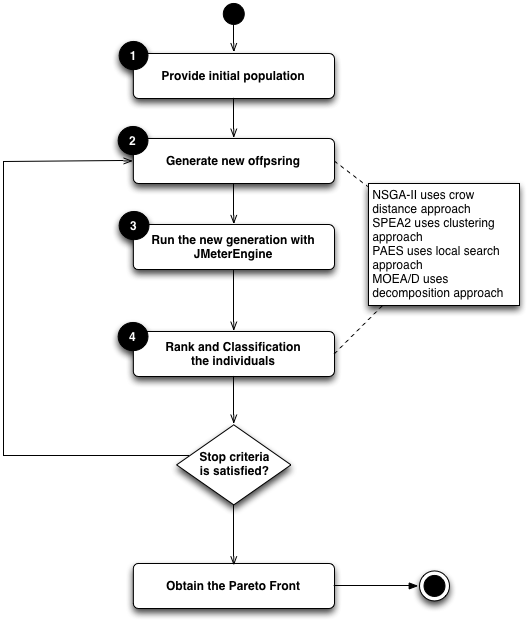
\includegraphics[width=0.8\textwidth]{./images/step3.png}
\caption{Flowchart of implemented algorithms}
\label{fig:flowchart}
\end{figure}


One experiments were performed to evaluate the use of multi-objective metaheuristics in search-based stress testing. The experiments use a SEDR adaptation algorithm. The experiment was undertaken with the JPetStore application with and without a noise reduction strategy. The maximum tolerated response time in the test was 1000 milliseconds.  The whole process of stress tests, which run for 5 days and 2226 executions, was carried out without the need for monitoring by a test designer. The tool automatically selected the next scenarios to be run up to the limit of 50 previously established generations by the algorithm. The hypervolume metric was used to compare the algorithms.  All values used in the hypervolume calculation were normalized. We used the emoa package of the R language to calculate the hypervolume.

\subsection{Experiment Research Questions}

The following research question is addressed:
\begin{itemize}
\item Which, among the four algorithms chosen, is the most suitable multi objective algorithm for the search-based test problem?
\end{itemize}

\subsection{Variables}

The independent variable is the algorithms: NSGA-II, SPEA2, PAES and MOEA/D. The dependent variables are the hypervolume of each algorithm.

\subsection{Experiment Hypotheses}

\begin{itemize}
\item With regard to the relevance of test results:
\begin{itemize}
\item $H_{0}$ (null hypothesis): The multi-objective with the higher value of hypervolume don't find the scenarios with higher response time and lower number of users.
\item $H_{1}$: The multi-objective with  the higher value of hypervolume find the scenarios with higher response time and lower number of users.
\end{itemize}
\end{itemize}

\begin{itemize}
\item With regard to hypervolume of multi-objective algorithms applied in the experiment:
\begin{itemize}
\item $H_{1}$: MOEA/D is the algorithm with the higher value of hypervolume in the experiments.
\item $H_{2}$: NSGA-II is the algorithm with the higher value of hypervolume in the experiments.
\item $H_{3}$: SPEA2 is the algorithm with the higher value of hypervolume in the experiments.
\item $H_{4}$: PAES is the algorithm with the higher value of hypervolume in the experiments.
\end{itemize}
\end{itemize}


\subsection{Experiment Results}

Table \ref{tab:hypervolume} shows the hypervolume value of each algorithm. Dimensionality shows the number of dimensions used in the calculation of hypervolume. For the hypervolume calculus, the values of the number of users and response time were transformed to the same scale. The highest hypervolume algorithm was the MOEA/D. 
Table \ref{tab:results2} presents the test scenarios found in the Pareto frontier of MOEA/D.

% Please add the following required packages to your document preamble:
% \usepackage[table,xcdraw]{xcolor}
% If you use beamer only pass "xcolor=table" option, i.e. \documentclass[xcolor=table]{beamer}
\begin{table}[!h]
\centering
\caption{Response time and number of users in optimal scenarios found with MOEA/D}
\label{tab:results2}
\begin{tabular}{|l|l|l|l|l|l|l|l|l|}
\hline
\rowcolor[HTML]{C0C0C0}
\textbf{N.} & \textbf{\begin{tabular}[c]{@{}l@{}}USERS\\ \end{tabular}} & \textbf{\begin{tabular}[c]{@{}l@{}}RESP \\ TIME\end{tabular}} & \multicolumn{1}{c|}{\cellcolor[HTML]{C0C0C0}\textbf{\begin{tabular}[c]{@{}c@{}}Dogs\\ Users\end{tabular}}} & \textbf{\begin{tabular}[c]{@{}l@{}}Enter\\ Catalog\\ Users\end{tabular}} & \textbf{\begin{tabular}[c]{@{}l@{}}Fish\\ Users\end{tabular}} & \textbf{\begin{tabular}[c]{@{}l@{}}Register\\ Users\end{tabular}} & \textbf{\begin{tabular}[c]{@{}l@{}}Add\\ Rem.\\ Cart\end{tabular}} & \textbf{\begin{tabular}[c]{@{}l@{}}Cart\\ Users\end{tabular}} \\ \hline
\ding{202}           & 1                                                        & 18                                                       &                                                           & 1                                                                 &               &                   &                                                                    &               \\ \hline
\ding{203}           & 5                                                       & 35                                                        & 1                                                          &                                                                &               & 3                 &                                                                    & 1              \\ \hline
\ding{204}           & 6                                                       & 50                                                        & 2                                                          &                                                                &               & 3                 &                                                                    & 1              \\ \hline
\ding{205}           & 7                                                       & 320                                                        &                                                           &                                                                &               & 3                 &                                                                    & 4              \\ \hline
\ding{206}           & 12                                                       & 410                                                        &                                                           &                                                                &               & 3                 &  5                                                                  & 4              \\ \hline
\ding{207}           & 22                                                       & 788                                                        &                                                           &                                                                & 7             &     7             &    3                                                                & 5              \\ \hline
\ding{208}          & 72                                                      & 1074                                                        & 17                                                        & 19                                                                & 14              &  11             &                                                                    & 11            \\ \hline
\ding{209}           & 89                                                      & 1396                                                        & 8                                                         & 7                                                               & 10             &                 & 29                                                                  & 35              \\ \hline
\end{tabular}
\end{table}


MOEA/D found two scenarios that approached the established service level for the experiment of 1000 milliseconds. NSGA-II  found a scenario with 49 users and response time of 685 and a scenario with 59 users and response time of 1138 milliseconds. Although the MOEA/D algorithm found the scenario with the lowest number of users with a time close to the service level, the NSGA-II found a scenario with more users with a response time closer to the service level. Figures \ref{fig:moeadnoise}, \ref{fig:paretofrontier2}, \ref{fig:spea2} and  \ref{fig:paes} present the Pareto frontier for each algorithm. Fig. \ref{fig:comparative3} presents a comparative graph between all the algorithms.

% Please add the following required packages to your document preamble:
% \usepackage[table,xcdraw]{xcolor}
% If you use beamer only pass "xcolor=table" option, i.e. \documentclass[xcolor=table]{beamer}
\begin{table}[]
\centering
\caption{Hypervolume by algorithm}
\label{tab:hypervolume}
\begin{tabular}{|l|l|l|l|}
\hline
\rowcolor[HTML]{EFEFEF} 
\textbf{ALGORITHM} & \textbf{HYPERVOLUME} & \textbf{DIMENSIONALITY} & \textbf{POINT DENSITY} \\ \hline
MOEA/D             & 10.185576            & 2                       & 7817.328935            \\ \hline
NSGA-II            & 7.541011             & 2                       & 7726.815663            \\ \hline
PAES               & 7.240581             & 2                       & 7758.493105            \\ \hline
SPEA2              & 5.539566             & 2                       & 7772.269274            \\ \hline
\end{tabular}
\end{table} 

\begin{figure}[h]
\begin{minipage}{.5\textwidth}
\centering
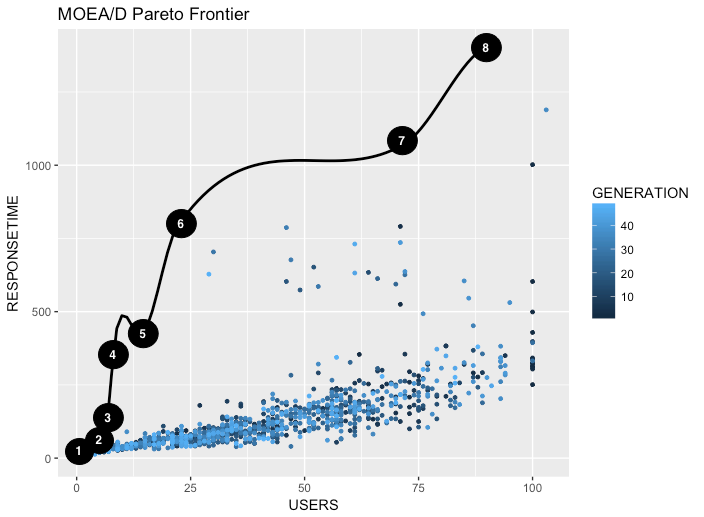
\includegraphics[width=1\textwidth]{./images/moeadnoise.png}
\caption{MOEA/D Pareto Frontier}
\label{fig:moeadnoise}
\end{minipage}
\begin{minipage}{.5\textwidth}
\centering
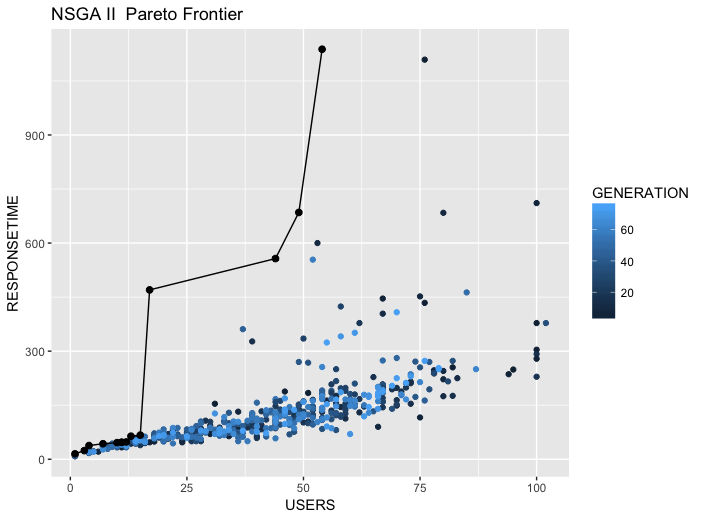
\includegraphics[width=1\textwidth]{./images/nsgaiinoise.png}
\caption{NSGA II Pareto Frontier}
\label{fig:paretofrontier2}
\end{minipage}
\end{figure}


\begin{figure}[h]
\begin{minipage}{.5\textwidth}
\centering
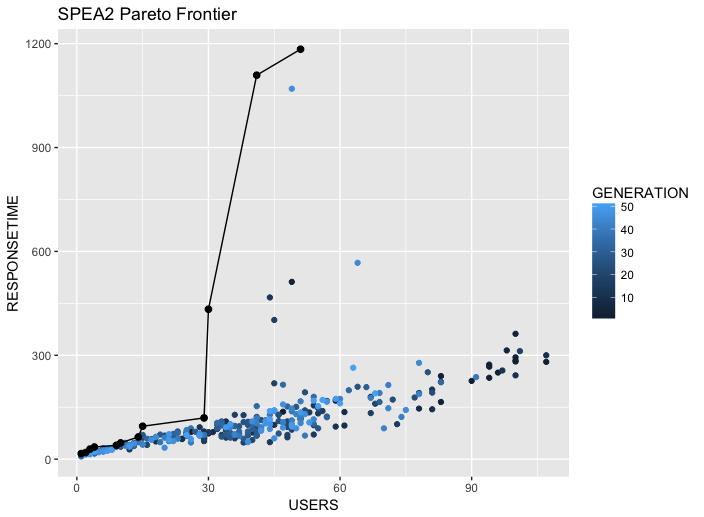
\includegraphics[width=1\textwidth]{./images/spea2noise.png}
\caption{SPEA2 Pareto Frontier}
\label{fig:spea2}
\end{minipage}
\begin{minipage}{.5\textwidth}
\centering
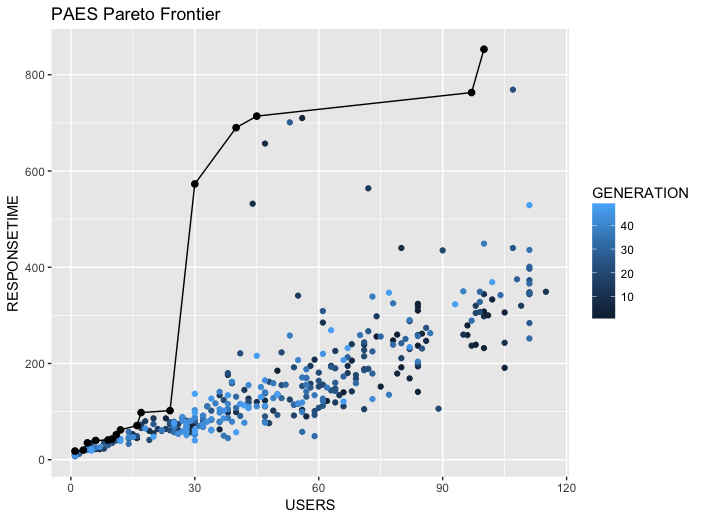
\includegraphics[width=1\textwidth]{./images/paesnoise.png}
\caption{PAES Pareto Frontier}
\label{fig:paes}
\end{minipage}
\end{figure}

\begin{figure}[h]
\centering
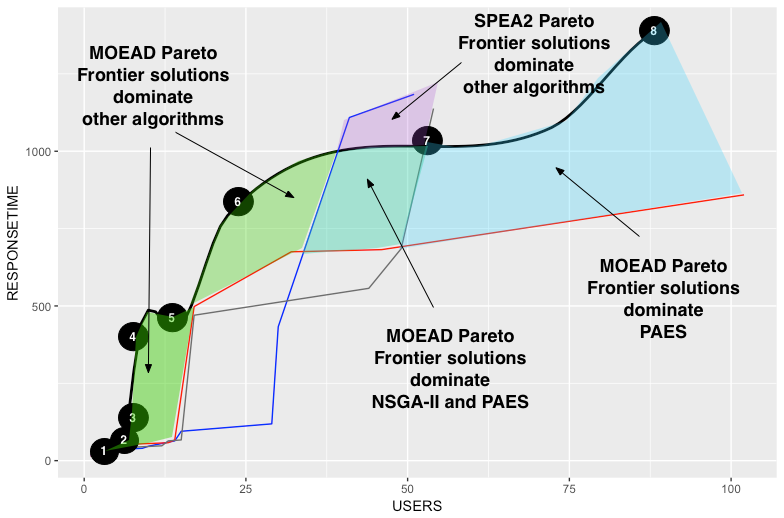
\includegraphics[width=1\textwidth]{./images/comparative3.png}
\caption{Comparative graph between MOEA/D, NSGA-II, SPEA2 and PAES Pareto Frontiers}
\label{fig:comparative3}
\end{figure}

\subsection{Experiment Conclusion}

The multi-objective with the higher value of hypervolume find the scenarios with higher response time and lower number of users. However, each algorithm presented relevant results for stress testing. MOEA/D was the algorithm with the highest hypervolume value.

\subsection{Threats to Validity}

Due to the non-deterministic nature of the problem, we do not guarantee that the same Pareto frontier will be found in different test executions. The workloads found by the MOEA/D algorithm  do not dominate all workloads found by all others algorithms.

\section{Conclusion}

This section presents our conclusions, shows some limitations, and proposals for future work. In this paper, we deal with the use of multi-objective metaheuristics in Search-based stress testing. A tool named IAdapter, a JMeter plugin for performing search-based load tests, was adapted. Several experiments were conducted to validate the proposed approach.

The use of multi-objective metaheuristics has made it possible to delimit a frontier where the response times are below the previously established service level. MOEA/D metaheuristics obtained the best hypervolume value when compared with NSGA II, SPEA2 and PAES. The experiments found  scenarios that contribute to the definition of the service level. There is a range of future improvements in the proposed approach. Also as a typical search strategy, it is sometimes difficult to ensure that the execution times generated in the experiments represent global optimum. More experimentation is also required to determine the most appropriate and robust parameters. Lastly, there is necessary to have an adequate termination criterion to stop the search process. Due to the pervasive and non-deterministic nature of the problem, we do not guarantee that the same Pareto frontier will be found in different test executions.  More experiments are needed to verify changes related to the Pareto frontier in different executions. The choice of fitness function can be a difficult step in Genetic Algorithms. The fitness function is still manually adjusted and additional studies need to be performed to get the best weight values for the fitness function.  Among the future works of the research, the use of different combinatorial optimization algorithms such as very large-scale neighborhood search is one that we can highlight. 



%The equation of the hypervolume is:


%\begin{equation}
%Hypervolume =  volume (U^{|Q|}_{i=1}  v_{i}  )
%\end{equation}






\section*{References}

\bibliography{mybibfile}

\end{document}